\section{Introduktion}

\begin{frame}{Introduktion}
	\begin{columns}
	\column[]{.7\textwidth}
	\begin{itemize}
		\onslide<1->{\item Data fra IGISOL ved Jyväskylä Universitet i Finland}
		\onslide<2->{\item Eksperimentet er foretaget i 2020}
		\onslide<3->{\item Undersøgelse af \li og \isotope[12]{B}}
		\onslide<4->{\item \isotope[7]{Li} + \isotope[2]{H} $\rightarrow$ \li + \isotope[1]{H}}
		\onslide<5->{\item \li $\rightarrow$ \ber + $e^- + \bar{\nu_e}$\\
		\ber $\rightarrow$ \isotope[4]{He} + \isotope[4]{He}}
		
	\end{itemize}
	\column[]{.3\textwidth}
	\includegraphics[width=\columnwidth]{../../Pictures/Finland.png}
\end{columns}
\end{frame}


\begin{frame}{Henfaldstyper}
	\begin{columns}
		\column[]{0.6\textwidth}
		\onslide<2->{Der findes to typer \be-henfald:}
		\begin{align*}
		\onslide<2->{&\beta^-:\quad n\rightarrow p + e^- + \bar{\nu_e}\\}
		\onslide<2->{&\beta^+:\quad p\rightarrow n + e^+ + \nu_e}
		\end{align*}
		\onslide<3->{\al-henfald er udsendelsen af en \al-partikel}
		\column[]{0.4\textwidth}
		\onslide<2-> 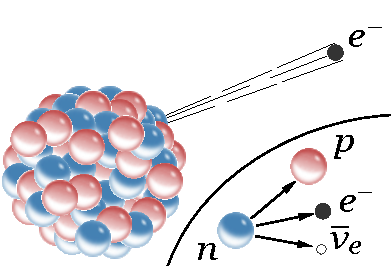
\includegraphics[width=\columnwidth]{../figures/Beta-minus_Decay.pdf}
		\tiny \url{https://en.wikipedia.org/wiki/Beta_decay}
		\onslide<3->\includegraphics[width=\columnwidth]{../../Pictures/aal.png}
		\tiny \url{https://en.wikipedia.org/wiki/Alpha_decay}
			
	
	\end{columns}
\end{frame}

\begin{frame}{Tilladte overgange}
	\onslide<2->{Total angular moment, paritiet og isospin: $J^\pi ; T$}
	\begin{equation*}
	\onslide<3->{\Delta J = 0,1,\quad \Delta T = 0, 1\quad \text{og}\quad \Delta \pi = 0}
	\end{equation*}
	\onslide<4->{
		\begin{figure}
			\centering
			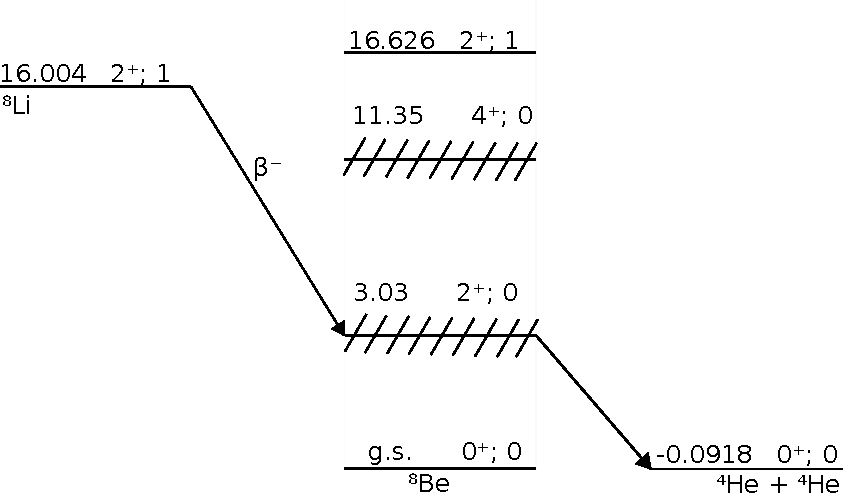
\includegraphics[width=.6\columnwidth]{../figures/DecayScheme.pdf}
		\end{figure}
	}
\end{frame}

